\documentclass[a4paper]{article}
\usepackage{INTERSPEECH2018}

\title{
       Detecting Double-Talks (Overlapping Speech) in Conversations\\
       using Deep Learning
}

\name{
       Abdullah,  % $^1$,
       Joachim K{\"o}hler,  % $^2$,
       Michael Gref  % $^2$
}

\address{
      % $^1$RWTH Aachen, Germany \\
      % $^2$
      Fraunhofer IAIS, Germany
}

% FIXME: Set appropriate email addresses
\email{
       abdullah.abdullahe@rwth-aachen.de,
       joachim.koehler@iais.fraunhofer.de,
       michael.gref@fraunhofer.de
}

\begin{document}

\maketitle

% ----------------------------------------------------------------------------------------- UTILS -
\newcommand{\outline}[1]{}  % outline notes that will not be exported.
\newcommand{\widom}[1]{}  % gudelines from https://cs.stanford.edu/people/widom/paper-writing.html

% -------------------------------------------------------------------------------------- ABSTRACT -
\begin{abstract}
\widom{
       - the problem,
       - the approach and solutions
       - the main contributions of the paper.
       - little if any background and motivation. address the experts.
       - factual but comprehensive.
}
We demonstrate training a Deep Convolutional Neural Network (DCNN) on real conversations to detect and segment naturally occurring instances of overlapping speech.
Using DCNNs affords us to use low-level log-scaled mel-spectrograms and to avoid previously necessary manual feature engineering.
We propose using conversational data from the Fisher English Corpus to properly train the DCNN while maintaining applicability to real conversational scenarios, as opposed to using artificially generated data.
To alleviate the then imposed challenge of severe class-imbalance, we report the improvements achieved by removing silence from the training objective and uniformly randomly under-sampling the majority class during training.
Simultaneously, we perform temporal smoothing using the Viterbi algorithm to enhance the final segmentations by utilizing the longer-term temporal patterns inherent to this phenomenon.
Our results promise the applicability of DCNNs for this task and urge for more research towards working with imbalanced classes, common in real-world problems, while using deep learning, especially in the domain of speech technologies.
\end{abstract}

% ----------------------------------------------------------------------------------- INDEX TERMS -
\noindent\textbf{Index Terms}:
overlapping-speech detection,
speech segmentation,
deep convolutional neural network,
conversation analysis,
class-imbalance issue,

% ---------------------------------------------------------------------------------- INTRODUCTION -
\section{Introduction}
\widom{
       - What is the problem?
       - Why is it interesting and important?
       - Why is it hard? (E.g., why do naive approaches fail?)
       - Why hasn't it been solved before? Or,
       - What's wrong with other solutions? How does mine differ?
       - What are the key components of my approach and results?
       - Any specific limitations of my approach?
       - Short yet detailed enough `Related Works` near the end, or make it as Section 2.
       - `Summary of Contributions` as the final para or subsection.
              - List the major contributions in bullet form,
              - Mention in which sections they can be found, doubling up as an outline.
}
% TODO: Figure out how to cite the author's names automatically

Overlapping speech, interchangeably referred to as double-talk in this paper,
occurs when more than one speakers speak simultaneously at a given instant.
A common occurrence in spontaneous conversations,
other participants often utter something while a speaker is already speaking,
possibly to demonstrate non-competitive acknowledgement (e.g. “mhm") or reaction (e.g. laughing),
or competitively interrupt having misjudged their turn to speak.
Its occurrence is of interest for Conversation Analysis in studying the
turn-taking management done by the participants of a conversation.
% ad-hoc mechanisms by which particpants manage turn-taking during a conversation.
While the frequency and durations of overlaps can vary depending on the situation,
overlaps are quite frequent and characteristically brief (predominently smaller than 1~sec)
during normal, spontaneous conversations (Figure~\ref{fig:dt-dist}),
making their manual annotation expensive and automatic detection challenging.

In the flagship scenario of spontaneous conversations,
the presence of double-talks is often detrimental to most automated speech technologies.
Speaker diarization systems, whose goal is to determine `who spoke when' in a conversation,
are penalized when they miss additional speakers during overlaps.
This penalty has become a major portion of the errors in the increasingly better
state-of-the-art performance of such systems,
so much so that Anguera et al. claim overlapping speech situations to be the `Achilles heel' of
speaker diarization systems when applied to meetings \cite{anguera_speaker_2012}.
Many other speech technologies (e.g. Automatic Speech Recognition)
rely on the speaker homogenous segmentations produced by a diarization system,
and have been reported to suffer from degaradation as well \cite{cetin_speaker_2006,RenalsDistantspeechrecognition2017}.

% ---------------------------------------------------------------------------------- FIG:DT-DIST -
\begin{figure}[t]
  \centering
  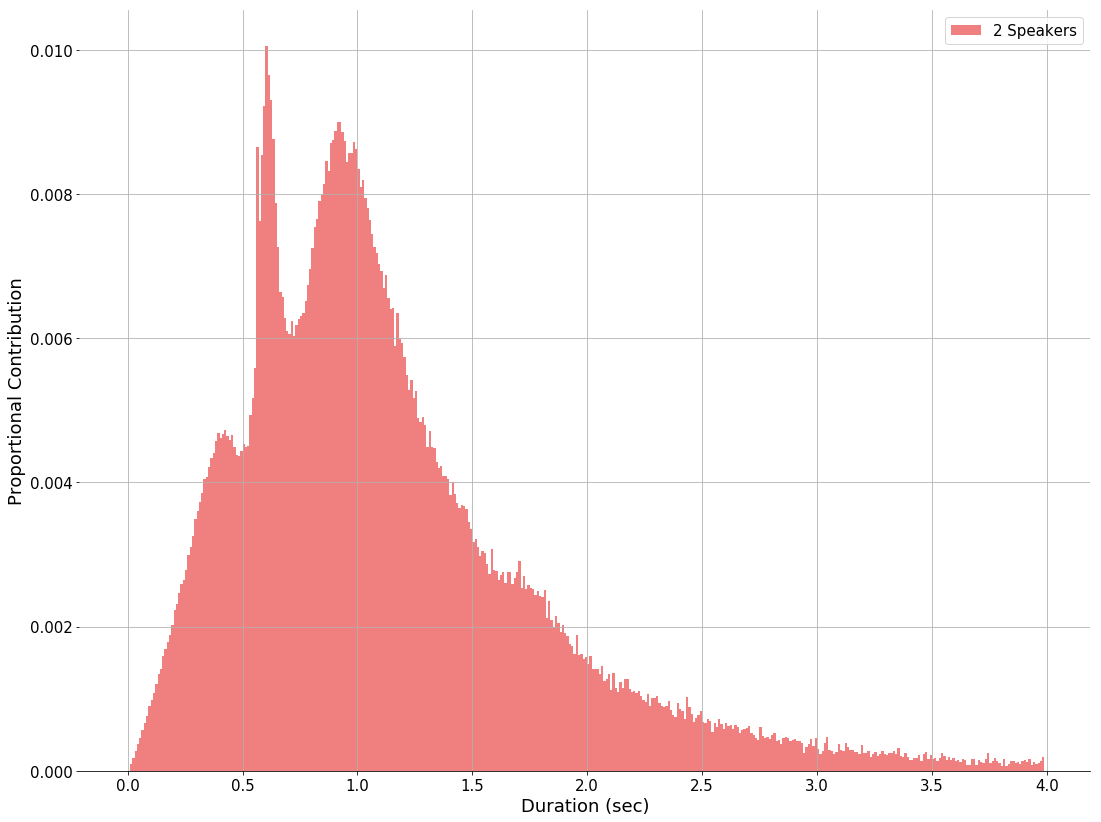
\includegraphics[width=\linewidth]{figures/dt-dist.png}
  \caption{Weighted histogram of durations of segments with double-talk in the Fisher English Corpus (Part 1).}
  \label{fig:dt-dist}
\end{figure}

Perhaps consequently, most previous attempts at detecting natural double-talks in conversations
have been made in lieu of improving speaker diarization systems.
% The most successful approaches propose employing a dedicated overlap detection system.
The problem has most commonly been formulated as performing frame-wise classification
for the presence of either
zero (i.e. silence), one, or more than one simultaneously active speakers,
and the solutions have been implemented in a GMM-HMM based framework
while engineering different combinations of acoustic features.
In general, using additional features from blah, blah, blah, or blah % TODO: T [text] summarize other features
have been found to improve overlap detection over using only spectral features.
Geiger et al. blah blah blah  % TODO: T [text] summarize LSTM-HMM approach.
The problem of overlap detection has remained largedly unsolved and
continues to present a steep trade-off between precision and recall of the system.

The most potent source of challenges in detecting natural double-talks is rooted in the inherent imbalance between the three classes.
It can be seen in Table X that in spontaneous conversations,  % TODO: T [tbl] Add table of segment and duration proportions.
while the individual occurrences of natural overlaps constitute a significant proportion of the total number of speaker-homogenous segmentations,
due to their predominently small duration, they account for the smallest proportion of individual frames.
Some studies have attempted to solve for this issue by training their proposed systems on artificially overlapped speech.  % TODO: T [ref, search] pyknogram paper, and the recent one, and any others
Shokouhi et al. reported better results when using their proposed Pyknograms as acoustic features for detecting overlaps under different noise conditions,
but their evaluations showed a discouraging dip in performance when the overlaps were less than 2\,seconds long \cite{shokouhi_teager_2017}.
In one of the recent proposals using a Deep Learning based method,
Andrei et al. reported achieving one of the better results in detecting overlaps of 500, 100 and 25\,millisecond \textit{window durations} \cite{AndreiDetectingOverlappedSpeech2017}
(it is unclear from the paper if this is also the temporal resolution (\textit{hop-size}) at which the predictions were made)
when MFCCs were combined with other acoustic features as inputs to a convolutional neural network.
However, no evaluations of such systems have been reported on detecting naturally occurring double-talks in real conversations.
Nevertheless, we believe that this approach of artificially increasing the training data has some pitfalls.
Most such approaches use with recordings of planned speech recorded in clean conditions as the raw data.
While artificially also adding noise helps in making the system more robust for real-world scenarios,
as done by Shokouhi et al. in their study \cite{shokouhi_teager_2017},
planned speech itself has very different properties than the spontaneous scenarios the system has to be applied to.
For example, certain vocal events like laughter, or certain utterances like those used as backchannels (e.g. “hmm", “m-hm"), which often and almost exclusively occur in natural conversations as overlapping utterances,
are difficult to account for in planned speech faithfully.
Speakers exhibit very different intonations, pace, disfluencies, etc. when they are speaking alone than when they are in a conversation.
We believe that the characteristics of double-talks,
with respect to typical duration, vocalization and content,
would be difficult to replicate in artificially overlaps created from planned single speaker speech.

% ------------------------------------------------------------------------------- TBL:ACTSPK-PERC -
\begin{table}[t] \label{tbl:actspk-perc}
  \caption{Percentage of segments and frames with different number of simultaneously active speakers in the $\sim \!\!\! \text{961\,hours}$ of Fisher English Corpus (Part 1).}
  \centering
  \begin{tabular}{crr}
    \toprule
    \textbf{Active Speakers}  & \textbf{Segments (\%)}  & \textbf{Frames (\%)}  \\ \midrule
    0                         & 20.39                   &  6.86                 \\
    1                         & 50.93                   & 79.61                 \\
    2                         & 28.68                   & 13.53                 \\
    \bottomrule
  \end{tabular}
  \vspace*{-\baselineskip}
\end{table}

Therefore, for our study, we have developed and evaluated our proposed system on naturally occurring double-talks in real telephonic conversations of the Fisher Corpus.  % TODO: T [ref] fisher paper, link
We have limited ourselves to work with mono-aural audio recorded at a sample rate of 8000\,Hertz,
in part forced by our choice of the dataset,
and in part motivated by our desire for the system to be applicable to almost all recording conditions.
Our system uses a Deep Convolutional Neural Network (DCNN) based automatic feature extractor and classifier working only on log-mel-spectrograms as inputs,
and hence avoids the need of previously prevelant feature engineering necessary for the task.
We present our proposals and systematic evaluation of different training strategies for solving the class imbalance issue and other inherent challenges posed by the problem.
Furthermore, we also evaluate the imporvements to our DCNN achieved by temporally smoothing its potentially noisy predictions
by using the Viterbi algorithm that incorporates longer-term temporal patterns that our DCNN is not able to learn on its own.

% -------------------------------------------------------------------------------------- APPROACH -
\section{Approach}
Our system performs frame-wise classification of the extracted acoustic features for a mono-aural audio into three classes based on the number of simultaneously speaking speakers:
zero (silence) $(no)$, one $(sp)$, or more than one (overlap) $(ov)$.
For our approach, we used 64\,dimensional $\text{log}_{10} \text{-scaled}$ melspectrograms (filter-banks)
extracted every 10\,milliseconds over a window of 32\,milliseconds (equivalent to 256 FFT-bins for 8000\,Hertz audio),
which have been shown to achieve better performance than MFCCs and pure spectrograms in various deep learning based acoustic models.  % TODO: T [ref] papers about fbank vs mfcc
For the purpose of reducing the mismatch between training and testing conditions, and as a crude noise reduction method,
we applied cepstral mean normalization on the extracted features.
However, we performed this on a chunk-by-chunk basis,
where the mean vector of a contiguous chunk of audio of roughly 2.5\,minutes duration was used to center all the vectors of that chunk.
This avoids the reliability issues with utterance level normalization by using long enough chunks,
while also avoiding impact of unrelated outliers if it were done over the entire datatset.
Additional variance normalization was not found to be helpful,
which is in line with other proposals using deep architectures.  % TODO: T [ref] against variance normalization in DL

The particular architecture of our DCNN is a heavily simplified version of VGG-net (Table X),  % TODO: T [ref] VGG-net
All trainings were performed using Adamax to optimize the categorical cross-entropy of the probability mass output for the three classes.
When constructing the input to our DCNN,
after the feature vectors have been normalized and before shuffled batches are created,
we add 10 frames each from immediately before and after a given frame to be classified (see inputs in Table X)  % TODO: T [tbl] DCNN arch
with the goal to provide additional contextual information to the classifier.
Our preliminary experiments showed that using fewer number of contextual frames gave relatively worse results,
while larger values came at significant computational cost.
We fixed our feature extraction pipeline and the DCNN's architecture for all our experiments in order to isolate the variables for the different training strategies discussed in later sections.

The frame-wise class posteriors class posteriors produced by our DCNN cannot exploit longer-term temporal patterns inherent to this problem with respect to typical duration of segments,
their probability of occurrence, etc.
The `raw' predictions obtained by simply applying frame-wise $argmax$ on the posteriors were observed to be noisy.
We therefore also experimented with applying the Viterbi algorithm \cite{rabiner_tutorial_1989} for decoding a temporally `smoothed' final segmentation and report its impact here.
The prior- and transition-probabilties used by the algorithm were calculated calculated on the training dataset and,
being class posteriors, the emission-probabilties were set to $1$.
Unlike most previous works,  % TODO: T [ref] papers that use OIP || non-ergodic HMM
we did not use an overlap-insertion penalty or manually modify the calculated probabilities.

% --------------------------------------------------------------------------------- TBL:DCNN-ARCH -
\begin{table}[t] \label{tbl:dcnn-arch}
  \caption{Architecture of the DCNN, and layers in each block.}
  \centering
  \begin{tabular}{ll}
    \toprule
    \textbf{Block}    & \textbf{Output's Shape}                         \\
                      & \tiny{(time, frequency, channel) or (size, )}   \\ \midrule
    Inputs            & (21, 64, 1)                                     \\ \midrule
    ConvBlk 1         & (9, 31, 64)                                     \\
    ConvBlk 2         & (3, 14, 128)                                    \\
    ConvBlk 3         & $\text{(256, )}^{\text{\tiny{global pooling}}}$ \\ \midrule
    FCBlk 1           & (512, )                                         \\
    FCBlk 2           & (128, )                                         \\
    FCBlk 3           & (32, )                                          \\ \midrule
    Outputs           & $\text{(3, )}^{\text{\tiny{softmax}}}$          \\
    \bottomrule
  \end{tabular}
  \begin{footnotesize}
    \begin{tabular}{l}
      \toprule
      \textbf{ConvBlk}   \\ \midrule
      Conv2D: (3, 3)     \\
      BatchNorm          \\
      ReLU               \\
      Dropout:  0.1      \\
      MaxPool2D: (2, 2)  \\
      \bottomrule
    % \end{tabular}
    % \begin{tabular}{l}
                         % \\
      \toprule
      \textbf{FCBlk}     \\ \midrule
      Dense              \\
      ReLU               \\
      Dropout:  0.1      \\
      \bottomrule
    \end{tabular}
  \end{footnotesize}
  \vspace*{-\baselineskip}
\end{table}

% ---------------------------------------------------------------------- TACKLING CLASS IMBALANCE -
\section{Tackling Class Imbalance}
While deep learning methods are extremely powerful,
they also suffer from degradation in performance as classic approaches do when the target classes are severely imbalanced.
There have been relatively few systematic studies to solve this problem in the context of deep learning.
Of ones that exist, most have concentrated on image classification related tasks.  % TODO: T [ref,search] DL with imbalance
Their proposals are often not so straightforward to apply on speech signals.
We discuss these approaches in the following sub-sections within the context of detecting overlapping speech.

% --------------------------------------------------------------------------------------- DATASET -
\subsection{Dataset}
%TODO: T [text] mention more clearly why dataset choice helps in tackling class imbalance
%             - natural vs. artificial overlaps
%             - large dataset, affording certain decisions that would be otherwise restricted
Previous works have on detecting overlapping speech in conversations have used data from meetings in datasets like AMI, NIST RT, ICSI, and others.  % TODO: T [ref] to meeting datasets
While they are appropriate, and perhaps the flagship scenario for evaluation,
these datasets pose extra challenging due to inconsistent and difficult recording conditions.
Previous works have reported to utilize only a subset of these datasets,
often to be comparable to other works,  % TODO: T [ref] papers that use meeting dataset for consistency
or due to limitations imposed by these conditions,
whose size we believed was not enough to appropriately train a DCNN with different strategies to handle the class-imbalance issue.
We decided to instead perform our study using the Fisher Corpus (Part 1),  % TODO: T [ref] Fisher paper
which consists of 5,850 telephone based conversations (amounting to more than 960\,hours) and is predominently used in conversational and large vocabulary speech recognition tasks in literature.  %TODO: T [ref] papers using Fisher
Most of these conversations have naturally occurring double-talks,
and the shear size of the available data makes certain simpler decisions later more affordable.
However, we limited ourselves to using only roughly 200\,hours of the dataset during trainings
(groups\,001\,to\,012, with 1299\,calls) and a fixed set of roughly 91\,hours for testing
(groups\,053\,to\,058, with 551\,calls),
mainly restricted by the training times for a DCNN.

Nevertheless, the Fisher Corpus imposes certain limitations of its own.
Being a telephone based conversation, the maximum number of overlapping speakers is strictly limited to two.
However, this scenario covers the majority of double-talk situations even when there are more than two participants.  % TODO: T [ref] Zelenak
All audios are sampled at 8,000\,Hertz, which could be a disadvantage,
but it is easier to reliably downsample audios of higher quality than doing the opposite.
In fact, by using mel-scaling with a fixed number of 64\,filter-banks,
our system can injest audio of any sample-rate,
although it may not be able to benefit from the better characteristics of higher quality audios.
Along the same lines, the raw recordings in the Fisher Corpus have two speaker specific channels which, when merged,
can only be used as mono-aural audios.
While using multi-channel audio could be better for performance,
but by supporting this least common denominator condition,
our system is applicable to most scenarios.

The most important problem with the dataset is the relative imprecision in annotation of the utterance boundaries.
As per the documentation,
these boundaries were not manually modified after they were determined by a speech activity detection system.   % TODO: T [ref] Fisher corpus
The properties of this speech activity detection system have not been mentioned,
but we found them to be less precise than ideal, especially in regions of small gaps.
These inaccuracies do not impact ASR systems as much as they would a system that needs to temporally localize events in the audio.
A powerful enough DCNN, when a large enough dataset is available to learn from,
may however be robust to such lack of precision,
and we did indeed observe this in many of our experiments.
Such inaccuracies exist in other datasets as well,
but they do not offer as much data for a deep learning method to comfortably learn from,
motivating us further to use the Fisher Corpus.
Nonetheless, these inaccuracies perhaps explain the peaks and tails in the segment length distribution in Figure X,  % TODO: T [fig] ovl segment dist
and can adversely impact the summary metrics used for evaluating the system, including the ones reported here.
We did not, however, modify the annotations before using them for the experiments reported here,
but we strongly recommend using a better speech activity detector to improve the available utterance boundaries for future works in this direction.

% -------------------------------------------------------------------- RE-BALANCING TRAINING DATA -
\subsection{Re-balancing Training Data}
The most common approach to tackle imbalanced classes is to rebalance the dataset that is seen by the system during training,
by either oversampling from the minority classes or undersampling from the majority classes.
When the available dataset is limited, oversampling the minority class is the most prevelant method,
and is often done by creating new examples of the minority class by transforming the existing examples in a way that is irrelevant to the task at hand (e.g. flipping an image) or other more sophisticated methods (e.g. SMOTE) to avoid overfitting.  % TODO: T [ref] paper on re-balancing, SMOTE
Such transformations are not straightforward to perform on audio signals.
Nevertheless, afforded by the size of the dataset available to us,
we instead chose to instead only evaluate undersampling the majority class during training for one of our experiments.
For this, we skipped frames with a single speaker's speech uniformly randomly when preparing the inputs for the DCNN,
such that the final ratio between single speech frames to overlapping speech was two-to-one
(we removed silence frames entirely when undersampling as explained in Section X.x).  % TODO: T [ref] removing silence section.
We chose the ratio to be two-to-one instead of one-to-one as an approximate method for presenting the DCNN with equal number of frames for each speaker alone and when overlapped.
A more sophisticated method for undersampling involves preferring examples of the majority near the boundaries with the minority class,
but we did not do this due to the imprecision in the boundary annotations (in most datasets).

% ------------------------------------------------------------------------------ REMOVING SILENCE -
\subsection{Removing Silence} \label{sec:rm-silence}
Silence, or lack of speech, is more easily discriminable than speech from any number of speakers,
whereas discriminating between speech produced by a single speaker and that produced by multiple speakers simultaneously, even in isolation, can prove difficult.
This problems becomes more severe due the imbalance disadvantaging overlapping speech more.
While training neural networks, this may result in situations where the classifier gets stuck in a steep local minima that is irrelevant, or even disadvantageous to double-talk detection.
Furtheremore, silence detection can be done by using much simpler methods than an expensive DCNN.  % IDEA: T [search,ref] more recent and better performing silence detection
Therefore, similar to many other previous works,  % TODO: T [ref] DT papers skipping silence
for a set of the experiments reported here,
we removed silence from the training objective based on the ground-truth label.
During evaluations of these experiments,
to enable temporal smoothing (Section X),  % TODO: T [ref] temporal smoothing section
we explicitly set the silence frames of the DCNN to be perfect predictions based on the ground-truth label,
instead of using an automated speech detector, to isolate the variables under study.

% ----------------------------------------------------------------------------------------- OTHER -
\subsection{Other}
Moving the threshold for assigning a class based on its priors is another method to tackle class imbalance.
Unfortunately, our experiments with this method were unstable and unreliable enough to be inconclusive, and hence are not reported here.
Perhaps this was due to the imbalance being too steep over a relatively few number of classes.
Another method is to modify the loss function during training based on misclassification penalties.
However, for stochastic gradient descent based deep learning,
this method is equivalent in impact to naive rebalancing of the training data,  % TODO: T [search,ref] cost-sensitive objective is rebalancing
and hence we did not investigate this method in our study.

% ----------------------------------------------------------------------------------- EXPERIMENTS -
\section{Experiments}
% ---------------------------------------------------------------------------- FIG:RAW-SMTH-PREDS -
\begin{figure*}[t] \label{fig:raw-smth-preds}
  \centering
  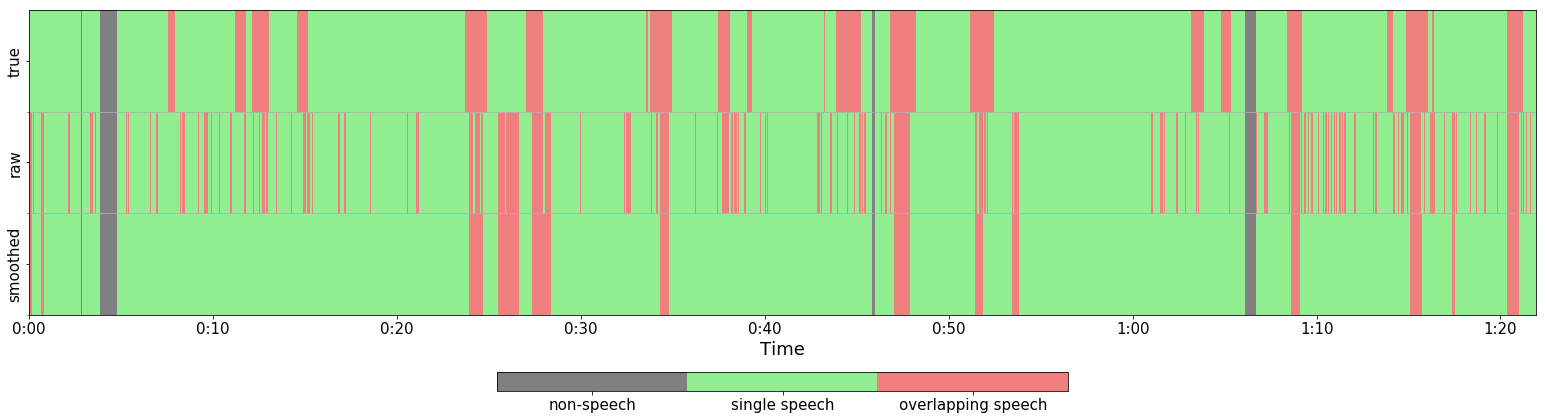
\includegraphics[width=0.8\linewidth]{figures/raw-smth-preds.png}
  \caption{True labels, raw-, and smoothed-predictions for part of a conversation, after training on rebalanced inputs.}
  \vspace*{-\baselineskip}
\end{figure*}

% ---------------------------------------------------------------------------------- TBL:RESULTS -
\begin{table}[t] \label{tbl:results}
  \caption{Class-wise precision $P$ and recall $R$ after different strategies, using $argmax$ `raw' or smoothed `smth` decoding.}
  \centering
  % \begin{tabular}{rrrrrrr}
  \begin{tabular}{ccccccc}
    \toprule
                & \multicolumn{2}{c}{\textbf{Baseline}}  & \multicolumn{2}{c}{\textbf{w/o Silence}}   & \multicolumn{2}{c}{\textbf{Rebalanced}}   \\
                &         raw      &         smth        &         raw      &         smth            &         raw      &         smth           \\ \midrule
    $P^{(no)}$  &         19.43    &         20.90       &         --       &         --              &         --       &         --             \\
    $R^{(no)}$  &         88.09    &         89.10       &         --       &         --              &         --       &         --             \\ \midrule
    $P^{(sp)}$  &         86.45    &         85.92       &         86.83    &         86.48           &         89.12    &         88.91          \\
    $R^{(sp)}$  &         82.15    &         83.61       &         99.05    &         99.79           &         88.39    &         96.69          \\ \midrule
    $P^{(ov)}$  & \textbf{81.30}   & \textbf{91.76}      & \textbf{68.87}   & \textbf{88.13}          & \textbf{35.25}   & \textbf{60.46}         \\
    $R^{(ov)}$  & \textbf{ 7.89}   & \textbf{ 5.05}      & \textbf{12.22}   & \textbf{ 8.82}          & \textbf{36.93}   & \textbf{29.55}         \\
    \bottomrule
  \end{tabular}
  \vspace*{-\baselineskip}
\end{table}

In the presence of imbalance, classwise precision and recall are more informative metrics than common measures like overall accuracy.
We report these metrics of the raw and smoothed segmentations at the frame level for all classes together so that any degradations in performance for other classes in strategies to improve the results on a particular target can be detected more clearly.
All evaluations were performed on the independent set of calls worth roughly 91\,hours of conversations as specified earlier.

In our preliminary experiments with several deep learning architectures and parameters,
we observed certain recognizable degenerate cases where the system failed to detect double-talks satisfactorily.
Some of the least powerful architectures predicted all fames to contain speech from a single speaker $(ov)$,
often with posterior probability as $1$, where not even temporal-smoothing could recover a useable result.
This is the classic case where a metric like overall accuracy would have mislead one severely.
A common degenerate case with moderately powerful architectures was where the system would perform robustly in detecting silence frames $(no)$ but will never detect any double-talk frames $(ov)$.
This unexpected speech activity detector demonstrated the extra disadvantage $(ov)$ face when $(no)$ is kept as part of the training objective, as discussed in Section\,\ref{sec:rm-silence}.
When some measures like threshold-moving were applied to tackle the class imbalance,
a common degenerate case involved extremely low precision for the $(ov)$ from what amounted to be random decisions for a frame to be from a single speaker $(sp)$ or multiple speakers $(ov)$.
Interestingly, in cases where silence was kept as part of the training objective,
this catastrophic level confusion still almost exclusively occurred between $(sp)$ and $(ov)$,
indicated by both a low precision for $(ov)$ ($P^{(ov)}$) and lower than 70\% recall for $(sp)$ ($R^{(sp)}$).

For a baseline performance measure of the proposed DCNN here,
we trained the system for 20 passes over the training set without rebalancing the classes and also kept silence as part of the training objective.
As tabulated in Table X,  % TODO: T [tbl,ref] table of all results
this baseline system did not detect silence frames with good precision $P^{(no)}$ resulting in many false-positives,
possibly due to the inadequacy of our crude denoising procedure.
This proved taxing for detecting double-talks, resulting in unsatisfactory recall $R^{(ov)}$,
perhaps due to the increased competition from silence of varying noise conditions.
However, the good precision of detecting overlaps $P^{(ov)}$ indicates that the DCNN did find some of the appropriate features representing double-talk situations.
The application of temporal smoothing improved $P^{(no)}$ and $P^{ov}$ by either removing impossibly short segments from the raw predictions or by filling in certain gaps (Figure X),  % IDEA: T [fig] true, raw, smoothed preds for baseline
but this also removed some otherwise correctly predicted frames, mostly disadvantaging $R^{(ov)}$ further.

We then trained the same DCNN for 20 passes over the same imbalanced training set,
but did not show it any silence frames, effectively removing it from the training objective and turning it into a binary classifier.
During evaluation, the silence frames were not removed from the input but,
interestingly enough, over the 91\,hours of our testing set,
none of the silence frames were detected as overlaps,
strongly suggesting that the DCNN had learned learned features that were specific to double-talks alone.
This resulted in improvements in $R^{(ov)}$, but came at a significant cost to $P^{(ov)}$ for the raw decisions.
The silence frames were manually set to perfect predictions to allow for temporal smoothing with the Viterbi algorithm,
and this smoothing regained the lost $P^{(ov)}$ with a relatively smaller cost to $R^{(ov)}$ than in the previous experiment.

For the final experiment presented here,
we trained our DCNN for 40 passes with a uniformly randomly undersampled single-speaker class as explained previously, while also removing silence from the training objective.
We doubled the number of passes for this experiment over the previous ones to avoid any under-fitting of the single-speaker class.
The evaluation of this DCNN on the testing set (which was obviously not rebalanced) showed an encouraging improvement in $R^{(ov)}$,
but with discouragingly high number of false positives in the raw predictions calculated with a naive $argmax$.
We however observed that most of these false positives occurred as noisy, impossibly short segments,
which were very adequately removed by the temporal smoothing procedure,
leading to a substantial improvement in $P^{(ov)}$ at a still smaller relative cost to $R^{(ov)}$.

% ----------------------------------------------------------------------------------- CONCLUSIONS -
\section{Conclusions}
We have demonstrated the possibility of using a DCNN for detecting natural double-talk by appropriately training on real conversations.
The challenge of class imbalance disadvantaging double-talks comes inherently with the use of real conversations for training.
Even without handling for this challenge, our DCNN learned some relevant features for double-talks,
demonstrating the power of this deep learning method.
We also showed that, in line with previous works,
removing silence from the training objective is useful in reducing the disadvantage against double-talks.
But the most benefitial strategy was to rebalance the training dataset.

The DCNN is capable of automatically learning the appropriate features for the task from the relatively low-level log-scaled melspectrograms, hence avoiding any heavy feature engineering.
Our decision to use the Fisher Corpus not only provided us with a large dataset for training and evaluation,
but also afforded us to choose random under-sampling of the majority class as the strategy for rebalancing the training data.
We believe that a system trained using this dataset and strategy is more readily and performantly applicable to detecting real conversations than one trained on artificial data.
A large enough dataset with higher quality audio and annotations would be better,
but we expect it to be an expensive one to acquire, if not build.

The performance our DCNN, however, is still less than ideal.
We expect a more powerful DCNN architecture to perform better for the problem.
However, we also demonstrated the weakness of DCNNs in exploiting longer-term temporal patterns by reporting the improvements achieved by temporal smoothing of the posteriors using the Viterbi algorithm.
We therefore expect improvements in performance by architectures that are capable of learning such patterns automatically (e.g. recurrent neural networks),
and perhaps even better when combined with convolutional neural networks based feature extractors.

The apparently steep trade-off between precision and recall that are the hall-mark of working with such heavily imbalanced classes was seen in the results very clearly.
There is a lack of comprehensive studies for tackling class imbalance when using deep learning,
especially in tasks related to speech technologies.
The task of detecting natural double-talks, as yet remaining an unsolved problem,
could be a worthwhile candidate for such studies,
if not also benefitting speech technologies that suffer in situations of overlapping speech.

% ---------------------------------------------------------------------------------- BIBLIOGRAPHY -
\bibliographystyle{IEEEtran}
\bibliography{dt-paper}
\end{document}
